%\documentclass{acm_proc_article-sp}
\documentclass{sig-alternate}
\newtheorem{definition}{Definition}
\usepackage{paralist}
\usepackage{url}
\usepackage{graphicx}
\usepackage{amsmath,amssymb}
\usepackage{listings}
\usepackage[utf8x]{inputenc}
\usepackage[dvipsnames]{xcolor}
\usepackage{tikz}
\usetikzlibrary{trees}


\newcommand\ednote[1]{\typeout{There is still an editor's note!!!}%
  \footnote{EDNOTE: #1}}
\newcommand\edbf[1]{\typeout{There is still an editor's note!!!}%
  \textbf{EDNOTE: #1}}

\def\collapse#1{\textcolor{blue}{\ensuremath{\mathord{\blacktriangleleft}
\mathord{#1}
\mathord{\blacktriangleright}}}}

% \DeclareUnicodeCharacter{B1}{\pm}
%% LANGUAGE      Markup definitions
\def\lstxml{
  \lstset{language=XML,
    basicstyle=\scriptsize,
    keywordstyle=\bfseries\ttfamily,
    identifierstyle=\ttfamily, 
    % commentstyle=\color{Brown},
    stringstyle=\ttfamily,
    showstringspaces=false,
    columns=[l]flexible, %% , basewidth={0.5em,0.4em}
    escapeinside={(@*}{*@)},
    deletekeywords={type,id}, % does not work!
    otherkeywords={encoding,
      mrow,math,mfrac,mi,msqrt,mo,mn,span,nobr,img,msup,maction,mtext}
  }
}
\def\lsthtml{
\lstset{language=html,
    basicstyle=\scriptsize,
    keywordstyle=\bfseries\ttfamily,
    showstringspaces=false,
    % otherkeywords={mfenced, open, close, separators, mrow, mi, mo, mn, math, 
    %   msup, role, parent, children, added}
}
}

\def\latex{\LaTeX}


\begin{document}
% \CopyrightYear{2019} 
% \setcopyright{acmcopyright}
% \conferenceinfo{W4A'16,}{April 11-13, 2016, Montreal, Canada}
% \isbn{978-1-4503-4138-7/16/04}\acmPrice{\$15.00}
% \doi{http://dx.doi.org/10.1145/2899475.2899494}


\title{Adaptable Accessibility Features for Mathematics on the Web}
  

\numberofauthors{3}
\author{
  \alignauthor {Davide Cervone}\\
  \affaddr{MathJax Consortium}\\
  \affaddr{Union College, NY}\\
  \email{\normalsize dpvc@union.edu}
  %
  \alignauthor{Volker Sorge}\\
  \affaddr{MathJax Consortium}\\
  \affaddr{University of Birmingham, UK}\\
  \email{\normalsize V.Sorge@cs.bham.ac.uk}\\
  %% Thanks does not seem to work.
}

\maketitle

\begin{abstract}
  Accessibility support for mathematical expressions has always been a
  challenging problem, not only since maths support is a niche area,
  but also because users have different assistive technology needs,
  have different levels of expertise, and work with material from many different
  subject areas. We present work towards making maths accessibility more
  adaptable to the reader's personal needs that is implemented in
  the MathJax library for rendering mathematics on the web. Since its
  inception, one of MathJax's goals was to provide accessibility support for
  visually and print impaired users. The new version 3 will provide both more
  features and more means of personalisation, and in particular, it provides
  adaptable combinations of highlighting,
  colorisation, and magnification techniques. Both Braille and speech output can
  be generated, with different speech rule sets allowing readers to flexibly change
  presentation and adaptation for improved interpretation of formulas in
  different subject areas, like Physics, Chemistry, and Logic.
\end{abstract}

\keywords{STEM Accessibility, Mathematics, MathJax}


\section{Introduction}

Assistive technology support for mathematical expressions has always been a
challenging problem --- one that is compounded not only by the fact that there exist
multiple markup languages in which to represent formulas, as well as multiple ways to
describe a given formula even in the same markup
language, but also that users have different needs, have different levels of
expertise, and work with material from different subject areas.

MathJax, a Javascript library for TeX-quality typesetting of Mathematics on the
web, has as its mission to provide not only visiual mathematics rendering on all
browsers and platforms, but also
accessibility support for blind and visually impaired people. This is achieved
either by supporting third-party assistive technology or, more recently, via
it's own integrated accessibility extensions. In MathJax's new version 3, the
accessibility extensions remain not only an important feature, but have been
considerably improved in terms of the information they can provide on formulas.

For expressions entered in {\LaTeX} format, an additional
emphasis is to provide better accessibility to advanced mathematical
material exploiting information gained from the original {\LaTeX} code, to provide
more appropriate speech for different areas of Mathematics, but also for subjects
like Physics, Chemistry and Logic.  Our aim is to ease the study of mathematics
for more people with visual impairments, as well as to encourage subject
specialists to contribute via better authored content, semantically meaningful
{\LaTeX} packages, and expert knowledge for speech generation.


Personalisation aspects:

\begin{itemize}
\item Automatic voicing of formulas
\item Interactive navigation with synchronised highlighting
\item Different collections of speech rules like MathSpeak and ClearSpeak
\item Nemeth Braille output
\item Subject specific voicing for advanced mathematics
\item Different magnification and zoom engines
\item Variety of highlighting styles
\end{itemize}

All this depends on a rich semantic representation of mathematical formulas.

Although MathJax can render the three most common markup language for
Mathematics --- {\LaTeX}, ASCIIMath, and MathML --- none of these has sufficient
semantic information to easily allow for the generation of meaningful speech,
explanations, or subject-specific highlighting.

Consequently MathJax relies on an improved semantic interpretation of formulas, which
is provided by the Speech Rule Engine (SRE)~\cite{}, a system that provides
speech generation for mathematical expressions given in presentation MathML.
SRE has been augmented with a number of additional features in recent years
that can be exposed in MathJax directly.  In addition, we have added new,
bespoke features in MathJax itself, which are mainly aimed at supporting readers
with low vision or learning impairments.

In this paper we describe the current state of math accessibility in MathJax,
presenting both features that exist in version~2.7~\cite{cervone2016towards} and
are novel to version~3. We will concentrate in particular on the novel adaptable
features and personalisation aspects of the new version.


\begin{figure}[t]
  \quad
  \begin{minipage}{.35\columnwidth}
\begin{lstlisting}[language=TeX,basicstyle=\scriptsize]
  ax^2 + b + c = 0
\end{lstlisting}
\begin{lstlisting}[language=XML,basicstyle=\scriptsize]
  <math>
    <mi>a</mi>
    <msup>
      <mi>x</mi>
      <mn>2</mn>
    </msup>
    <mo>+</mo>
    <mi>b</mi>
    <mi>x</mi>
    <mo>+</mo>
    <mi>c</mi>
    <mo>=</mo>
    <mn>0</mn>
  </math>
      \end{lstlisting}
    \end{minipage}
  \qquad
\begin{minipage}{.6\columnwidth}
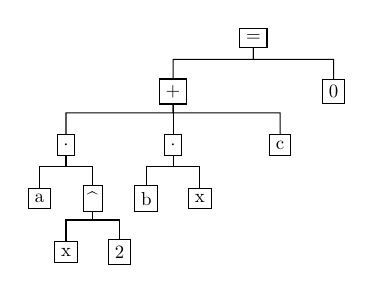
\begin{tikzpicture}[scale=.68, transform shape,
  level 1/.style={level distance=.8cm}
  ]
  \node[draw] {=}
  [grow via three points={one child at (0,-1.25) and two children at
(-1.5,-1) and (1.5,-1)}, edge from parent fork down]
  child {node[draw] {+}[grow via three points={one child at (0,-1) and
two children at (-1,-1) and (1,-1)}, edge from parent fork down]
  child {node[draw] {$\cdot$}[grow via three points={one child at
      (0,-1) and two children at (-.5,-1) and (.5,-1)}, edge from parent fork 
down]
    child {node[draw]{a}}
  child {node[draw] {$\,\widehat{}\,$}[grow via three points={one
      child at (0,-1) and two children at (-.5,-1) and (.5,-1)}, edge from parent 
fork
    down]
    child {node[draw]{x}}
    child {node[draw]{2}}}
        }
  child {node[draw] {$\cdot$}[grow via three points={one child at
      (0,-1) and two children at (-.5,-1) and (.5,-1)}, edge from parent fork 
down]
    child {node[draw]{b}}
    child {node[draw]{x}}
        }
  child {node[draw]{c}}
        }
  child {node[draw] {0}}
  ;
\end{tikzpicture}
  \end{minipage}
  \caption{Quadratic equation $ax^2 + bx + c = 0$ in {\LaTeX}, presentation
    MathML, and as a semantic term tree.}
  \vspace*{-.3cm}
  \label{fig:semantic-tree}
\end{figure}

\begin{figure*}[h!]
  \begin{lstlisting}[language=XML,basicstyle=\scriptsize\tt]
<mjx-container class="MathJax" jax="CHTML" display="true" hasspeech="true" tabindex="1">
  <mjx-math type="relseq" role="equality" id="16" children="15,10" content="9"
            aria-label="a x squared plus b x plus c equals 0" 
            speech="a x squared plus b x plus c equals 0">
    <mjx-mrow type="infixop" role="addition" id="15" children="12,14,8" content="4,7" parent="16"
              speech="a x squared plus b x plus c">
      <mjx-mrow type="infixop" role="implicit" id="12" children="0,3" content="11" parent="15"
                speech="a x squared">
        <mjx-mi class="mjx-i" type="identifier" role="latinletter" font="italic" id="0" parent="12" speech="a">
          <mjx-c c="a" />
        </mjx-mi>
        <mjx-mo class="mjx-n" type="operator" role="multiplication" id="11" parent="12" speech="times">
          <mjx-c c="2062" />
        </mjx-mo>
        <mjx-msup type="superscript" role="latinletter" id="3" children="1,2" parent="12" speech="x squared">
          <mjx-mi class="mjx-i" type="identifier" role="latinletter" font="italic" id="1" parent="3" speech="x">
            <mjx-c c="x" />
          </mjx-mi>
          ...
  </mjx-math>
</mjx-container>
\end{lstlisting}
\caption{Rendered quadratic equation in MathJax v3 with embedded
  semantic tree and speech.}
\label{fig:rendered}
\end{figure*}



\section{Semantic Enrichment}
\label{sec:semantic-enrichment}

One of the main challenges to produce useful assistive technology support in
MathJax is the lack of semantic information in most standard mathematical markup
notations. Formulas are usually given in format that are geared towards visual
representations, such as {\LaTeX}, ASCIIMath, or MathML, with
{\LaTeX} being clearly prevalent on the majority of webpages. Similarly, MathJax was
originally designed exclusively for displaying formulas, offering a number of
different rendering solutions, such as HTML with CSS or SVG output.
Figure~\ref{fig:semantic-tree} presents two standard ways of representing the
quadratic equation $ax^2 + bx + c = 0$, in {\LaTeX} on the top and in MathML on
the left. Both are given in a very flat structure, that only lends itself to a
linear representation. This can be sufficient to create speech, but in
general, is not enough to create good mathematical explanations and interaction
support.

Consequently, the first step towards accessibility support in MathJax is by
imposing a semantic interpretation on a given math expression and generating a
tree representation that can be embedded into rendered MathJax expressions to
ensure a similar user experience across browsers. The idea of the semantic
interpretation is an extension of the heuristics implemented in the screen
reader ChromeVox~\cite{Sorge14} and further developed in the context of
MathJax~\cite{cervone2016towards}, which effectively rewrites a flat expression
into a term tree structure by first interpreting the basic nature of symbols, and
propagating this through the expression to determines the scope of operators,
relations, etc. Figure~\ref{fig:semantic-tree} presents this transformation for
the example of the quadratic equation $ax^2 + bx + c = 0$, which is rewritten
from either its MathML or {\LaTeX} form into its semantic interpretation on the
right.

The resulting semantic tree can be understood as an orthogonal view of the
mathematical expression. To exploit it, we embed it using \texttt{data} attributes
into the DOM elements that represent MathJax's rendering of the equation
regardless of the choice of a particular rendering solution. MathJax offers
several different output formats, where
expressions in the DOM are collections of \texttt{div} and \texttt{span}
elements, HTML5 custom elements, or SVG graphics elements. These collections
often don't correspond well to the mathematical structures they represent.
Figure~\ref{fig:rendered} contains the rendered DOM expression as output by
MathJax v3. It uses HTML5 custom elements and \texttt{data} attributes, where
\texttt{type}, \texttt{role}, \texttt{id}, \texttt{parent}, \texttt{children}, \texttt{content}, and \texttt{speech} are
actually data attributes, with a \texttt{data-semantic-} prefix. This has been
omitted in the figure to preserve space and improve readability. The actual
semantic tree structure is represented via the \texttt{id}, \texttt{parent}, \texttt{children},
and \texttt{content} attributes. Note that both the use of custom elements and data
attributes provide a fast and standardized means of retrieving information from
the DOM that is fully consistent with HTML5 practices.


\section{Overview of Accessibility Features}
\label{sec:at-solution}

The assistive technology extension that we have built for MathJax is mainly
aimed at supporting users with reading disorders, such as dyslexia, and visual
impairments. However, some aspects if it could also be used as a general aid for
readers unfamiliar with the content or for learners at different levels. We
summarize the main features in this section.

\subsection{Speech Output}

One main emphasis of the assistive technology extension is to support
screen-reader users, but make them independent of their particular
screen-reader's Math capabilities. MathJax exploits the features of the
speech-rule engine~\cite{Sorge14,SRE-release-3} that generates the initial semantic-tree
transformation to also provide aural rendering for mathematical
expressions. Speech-string computation is based on the embedded semantic
tree. Speech strings for a formula are either generated on the fly when running
MathJax in a browser client, or pre-computed by a page author, e.g.,
if formulas are embedded as pre-rendered elements into a page.

To expose the speech strings to a screen reader, MathJax uses two main
techniques.  Firstly, a description of an entire formula is given in the ARIA
label at the top level of the DOM structure representing the expression.
Figure~\ref{fig:rendered} demonstrates the ARIA label embedding as well as the
use of a custom data attribute for speech. The latter allows us to aurally
render not only the entire formula but each of its subexpressions, which is
exploited during user interaction with the formula, as discussed below.  For
this purpose, MathJax introduces a dedicated assertive ARIA live region into the
DOM and updates it with the desired speech output. Content changes in the live region
are picked up by screen readers and spoken. This is a feature that is
particularly in line with MathJax's mission to support mathematics
rendering in all browsers and on all platforms, working with any modern screen
reader that supports live regions.


\subsection{Tactile Output}

In addition to speech output, SRE now provides generation of Braille
output using Unicode Braille symbols. It currently supports translation of
expressions into Nemeth Braille~\cite{nemeth} only, but we plan to support
additional Math Braille styles in the future. In MathJax we can make use of this
feature by computing Nemeth output as a further rendering mode in parallel to
visiual and speech output.

Unfortunately, there is currently no easy way to get tactile output to the user
during regular reading, as most screen readers translate text internally into
Braille, which is not necessarily helpful for Mathematics that needs specific
Braille formats. In particular there is no way to inject Braille directly into
alt text or aria labels for screen readers to simply pick it up and pass it on.
However, during user interaction with a formula, MathJax takes control so that
Braille content can be exposed. This is similar to speech: The unicode Braille
is simply pushed into a second live region which can be picked up by a screen
reader that directly pushes it onto a connected Braille display.



\subsection{Visual Aids}

Since MathJax has full control over the rendering of a mathematical expression
in the browser, it can offer a number of assistive techniques based on visual
alteration and enhancement of formulae. While these are mainly geared towards
supporting readers with low vision or other print impairments like dyslexia,
they can also help a general audience in improved understanding for formulas and
their structure.

\paragraph{Highlighting and Contrast}

Mathematical expressions generally are large collections of mostly unconnected
symbols in a two-dimensional layout that can be particularly daunting for
readers with dyslexia.  Reading comprehension can be supported, however, by a
choice of high-contrast colors~\cite{rello2012optimal} and selective
highlighting~\cite{jones2008strategies}. We realize this in MathJax by offering
changes of fore- and background colors, and selective highlighting of
sub-expressions of a complex formula. In the case of the former, the entire
formula is simply colored to simulate a colored overlay to provide high-contrast
in itself or to offset it from the surrounding text.  For the latter, we again
exploit the semantic structure of the formula to provide a more meaningful
highlighting of sub-formulas. Below is a simple example of progressive shading
for the quadratic equation:

\def\cb#1{\colorbox{yellow}{\ensuremath{\!\!\displaystyle#1\!\!}}}
\def\cc#1{\colorbox{GreenYellow}{\ensuremath{\!\!\displaystyle#1\!\!}}}
\[\cc{\cb{ax^2} + \cb{bx} + \cb{c}} = \cc{\rule[3ex]{0pt}{0pt}0}\]

In practice, sub-expressions are highlighted when hovering over them with the
mouse pointer, or by switching highlighting on permanently. This can be
recursively refined for sub-expressions, e.g., hovering on the denominator or
numerator of a fraction only. For permanent highlighting, the opaqueness of the
background gradually increases in nested sub-expressions. Nevertheless, in large
expressions, highlighting is of limited utility in getting an overview of the structure
of a formula; to aid this further, we introduce a technique for
structural abstraction in the next section.

\paragraph{Structural Abstraction}

The idea of structural abstraction is to assist readers by simplifying the
structure of the formula initially and letting them individually explore the
equation by manually expanding selected sub-expressions. Below is an example of
structural abstraction for the quadratic equation, where the sum on the
left-hand side is collapsed into a single addition symbol that can be expanded
to the full sum by clicking on it.

\[\collapse{+}=0\]

While in this case the abstraction is fairly trivial (for some more complex
examples see~\cite{cervone2016towards}), for large or complex formulas and
equation systems, abstraction can often significantly simplify the visual
appearance, leading to less cognitive load for a reader, as well as a better
understanding of the basic structure of an expression. In addition, abstractions
can aid in producing concise speech descriptions via summarisation of formulas
or parts thereof. This can be particularly important for presenting formulas
inline in mathematical texts, where a reader might want to understand the whole
text without having their reading flow constantly interrupted by every formula
being spoken in minute detail. In addition, visual abstraction can be helpful in
presenting mathmatics on small form factor displays by adapting formulas to the
page reflow to avoid the need for left right panning of a page.


\paragraph{Formula Colouring}

An alternative means to providing support to readers with print impairments is
to heighten the contrast of elements within a formula itself. This effectively
amounts to offsetting neighbouring symbols as much as possible with contrasting
colors. While this could be done in a linear fashion, exploiting the semantic
tree structure allows for a similar effect while also offering the possibility
of retaining the same or similar colors for the same or similar operations. A
tree colouring example for the quadratic equation is given below:
\[\color{blue}a \color{OliveGreen}x^2 \color{red}+ \color{blue}b
  \color{OliveGreen}x \color{red}+ \color{blue}c \color{black}= \color{magenta}0\]


\paragraph{Magnification}

\edbf{Rewrite to contain the new magnification.}

While changing contrasts can already help low-vision users, many rely on screen
magnification to read content.  MathJax supports magnification in multiple ways:
standard browser zoom is supported by re-rendering mathematics at the new size.
MathJax also provides global scaling settings to enlarge all math
elements at once.  Individual math expressions can be further magnified using a
``lens'' that ordinarily offers a zoom window on top of an expression, with
scrolling to pan across the entire zoomed expression. Exploiting the semantic markup,
this lens can be restricted to particular sub-expressions only, as for instance
in the example below.


\edbf{Put in example.}


\subsection{Interactive Features}

Since mathematical formulas are generally of a complex nature, and already a
small formula can make for a complex utterance, just listening to an expression
once is generally not enough for comprehension. Therefore, it is particularly
important to provide the reader with a means of engaging with formulas
interactively. MathJax offers an interface for interactive exploration of
mathematical expressions that allows a reader to step through sub-expressions.
Technically, this is realized by giving each math expression an ARIA role of
\texttt{application}, and upon entering an expression, the user can walk it
using the cursor keys.

During this exploration, many of the previously described features can be
restricted to sub-expressions as well. Speech strings can be
computed for all sub-expressions and voiced by updating the ARIA live region
introduced in the DOM. Similarly highlighting as well as magnification can be
synchronised to the exploration using CSS techniques.

It is important to note that the walking is not done in a linear
``left-to-right'' fashion, but instead follows the embedded semantic tree
structure. Thus starting with the entire expression, the next lower level
consists, for instance in the case of the quadratic equation, of the sum on the
left hand side of the equation, the equality sign and the $0$ on the right.  The
sum can then be further explored allowing the reader to then step through the
single summands from left to right, and so on.  Note also that this
ensures that the user experience of exploring a structure is the same regardless
of the specific renderer used even though their underlying DOM trees differ.
In addition to this, MathJax also provides the ability to
query the position of elements in a formula, means to summarise the expression currently
highlighted, cursor virtualisation, as well as special navigation modes for
matrices and equation systems.


\section{Adaptation and Personalisation}
\label{sec:challenges}

\subsection{Altering Speech}

MathSpeak vs ClearSpeak

Example: Quadratic formula

\subsection{Domain Specific Semantics}

\begin{itemize}
\item Domain specific interpretation from {\LaTeX}
\item Domain adaptation by choice of heuristics
\item Example: Bra-ket notation.
\end{itemize}



\section{Conclusions}
\label{sec:conc}

\edbf{Rewrite entirely or just point to future work.}

We have presented the new accessibility features of MathJax that aim to
transform MathJax into a universal rendering solution supporting all readers,
regardless of their assistive needs. The features are based on a improved semantic
enrichment procedure for Presentation MathML, which not only ensures a uniform
user experience across platforms and output formats, but also shows promise
for more advanced AT techniques in the future. Some of these features are available
as extensions to MathJax version~2, but all will be included as part of the core
distribution for MathJax version~3.

%   We therefore believe that our work can be
% significantly expanded, by
% \begin{inparaenum}[(1)]
% \item enhancing the precision of the semantic analysis, 
% \item adding subject specific rules, or 
% \item harvesting semantics from surrounding context.
% \end{inparaenum}

Although we have not yet had the opportunity to do extensive user testing, since
our code is developed publicly on our GitHub repository, we have already had
some user feedback, in particular from specialists, where initial reactions have
been positive. Additional end-user testing was enligthening: users struggled 
with lack of live-regions support in their AT and the complexity of the 
application. Feedback indicates that options for additional speech styles and 
semantics will be beneficial. 
We spent a significant effort on
technical testing in order to make the solution compatible with the most common
assistive technology solutions, and
strongly believe that these experiences and
observed shortcomings should serve as a foundation for the future development
of standards, tools, and general accessibility solutions for STEM content on the
web. 


\subsection*{Acknowledgements}
Simons Foundation, Big Ten Academic Alliance, anyone else?  Sloan foundation for earlier work?




\begin{thebibliography}{1}\small

\bibitem{voiceover}
Voiceover.
\newblock \url{apple.com/accessibility/osx/voiceover}.

\bibitem{HTML5}
% R.~Berjon, S.~Faulkner, T.~Leithead, E.~Doyle Navara, E.~O'Connor, S.~Pfeiffer, I.~Hickson.
\newblock {HTML} v5.0.
\newblock W3C recom., 2013.
\newblock \url{www.w3.org/TR/html5}.

\bibitem{MathML3}
D.~Carlisle, P.~Ion, R.~Miner.
\newblock {MathML} v3.0.
\newblock W3C recom., 2010.
\newblock \url{www.w3.org/TR/MathML3}.

\bibitem{MathJax2.5}
\newblock {MathJax} v2.5, 2014.
\newblock \url{www.mathjax.org}.

\bibitem{jones2008strategies}
R.~Jones.
\newblock Strategies for reading comprehension: Selective underlining, 2008.

\bibitem{MathSpeak}
A.~Nemeth.
\newblock Mathspeak.
\newblock \url{www.gh-mathspeak.com}, 2005.

\bibitem{rello2012optimal}
L~Rello and R~Baeza-Yates.
\newblock Optimal colors to improve readability for people with dyslexia.
\newblock In {\em Text Customization for Readability Symposium}, 2012.

\bibitem{soiffer2005mathplayer}
N.~Soiffer.
\newblock Mathplayer: web-based math accessibility.
\newblock In {\em 7th Computers and Accessibility Conf.}, 2005. ACM.

\bibitem{Sorge14}
V.~Sorge, C.~Chen, T.V.~Raman, D.~Tseng.
\newblock Towards making mathematics a first class citizen in general screen
  readers.
\newblock In {\em 11th Web for All Conf.}, 2014. ACM.

\bibitem{Sorge15}
V.~Sorge, M.~Lee, S.~Wilkinson.
\newblock End-to-end solution for accessible chemical diagrams.
\newblock In {\em 12th Web for All Conf.}, 2015. ACM.

\end{thebibliography}

% \pagebreak
% \begin{itemize}
% \item first comment: "My main concern with the paper is the lack of evaluation of the proposed features. Although extensive testing is listed as one of the challenges, due to the lack of adequate tools, a few evaluations based on user observation would already provide invaluable feedback to help improve each feature and MathJax as a whole."
% \item Peter: user feedback was sought but is still being overshadowed by the limitations of the platform (see below)
% \item Peter: user feedback negative in this sense: too hard to understand when to drop out of modes, how to interact, how to know AT well enough to get the benefits
% 
% \itme Limited end user testing was more. Users struggled with lack of 
% live-regions support and the complexity of the application. Inexperience with 
% voicing and exploration of mathematical content made it difficult for them to 
% assess the quality of the results.
% 
% \item second comment "it would have been even stronger had it been able to more generally extrapolate from this experience to the sorts of challenges that would be encountered in adding analogous extensions to other interfaces."
% \item Volker: write about generalization for similar STEM apps -- quote V's chemistry paper
% \item Volker: write what would be nice  / good to know for similar endeavors
% \item Peter: unclear implementation status of aria live regions (sometimes not announced, AT not leaving browse mode), AT feature "jump to last heard application and put focus on it; resume after leaving app" (in browse mode ) b/c in browse mode you pass an application with a label and you can't access it o
% \item Volker: automated tests and CI simply not possible 
% \item Peter: therefore increased development and maintenance costs, slowdown in feeding research into practice
% 
% \item third commment: "In fact, the practical approach of the paper is obvious, but it could excite more partners and collaborators, of the issues be shown as investigations or even if they were presented in a more scientific and contextualized way (for example, provoking developers to think about the levels of solutions they could be involved) ."
% \item Volker: see it as application engineering
% \item Volker: building rich web apps (menus, games) but apps on enriching content
% \item Volker: e.g., VO explains "applcation: press controle+alt+option+... to enter" but doesn't work becaue you're in the wrong mode.
% \end{itemize}

\end{document}


%%% Local Variables:
%%% mode: latex
%%% TeX-master: t
%%% End:
